\documentclass[article,aoas,preprint]{imsart}

\usepackage[nofiglist, nomarkers]{endfloat}
\usepackage{algorithm}
\usepackage{graphicx}
\usepackage{amsmath}
\usepackage{amssymb}
\usepackage{amsfonts}
\usepackage{amsthm}
\usepackage{xfrac}
\usepackage{float}
\usepackage{fullpage}
\RequirePackage[colorlinks,citecolor=blue,urlcolor=blue]{hyperref}

% override imsart settings for final project
\startlocaldefs
\setattribute{title}{size} {\fontseries{bx}\fontsize{14}{16}\selectfont\mathversion{bold}\spaceskip.5em}
\setattribute{journal}{name}{PH240F: Statistical Genomics II}
\setattribute{author}{prefix}{}
\setattribute{volume}{title}{Spring 2014---Final Project}

\makeatletter
\let\@fnsymbol\@arabic
\makeatother
\numberwithin{equation}{section}
\theoremstyle{plain}
\newtheorem{thm}{Theorem}[section]
\newtheorem{lemma}{Lemma}[section]
\newtheorem{definition}{Definition}
\newtheorem{Rule}{Rule}
\newtheorem*{notation}{Notation}
\endlocaldefs

% my standard setup 
\newcommand{\der}[2]{\frac{d #1}{d #2}} % for derivatives
\newcommand{\V}[1]{\ensuremath{\mathbf{#1}}} % for vectors
\newcommand{\gv}[1]{\ensuremath{\mbox{\boldmath$ #1 $}}} % for vectors of Greek letters
\newcommand{\pd}[2]{\frac{\partial #1}{\partial #2}}  % for partial derivatives
\newcommand{\grad}[1]{\gv{\nabla} #1} % for gradient
\newcommand{\reals}{\mathbb{R}}
\newcommand{\ints}{\mathbb{Z}}
\newcommand{\blank}{\underline{\hspace*{1in}}}
\newcommand{\PMF}{\mathrm{PMF}}
\newcommand{\PDF}{\mathrm{PDF}}
\newcommand{\CDF}{\mathrm{CDF}}
\newcommand{\N}[2]{\mathcal{N}\left(#1,#2\right)}
\newcommand{\empavg}[2]{\frac{1}{#1}\sum_{i=1}^{#1}\left[#2\right]}
\newcommand{\E}[1]{{\rm I\kern-.3em E}\left[#1\right]}
\newcommand{\Var}[1]{\mathrm{Var}\left[#1\right]}
\newcommand{\Cov}[1]{\mathrm{Cov}\left[#1\right]}
\def\ci{\perp\!\!\!\perp}
\newcommand{\argmax}[1]{\underset{#1}{\operatorname{argmax}}}
\newcommand{\argmin}[1]{\underset{#1}{\operatorname{argmin}}}
\newcommand{\iid}{\stackrel{\mathrm{iid}}{\sim}}
\newcommand{\logit}[1]{\operatorname{logit}({#1})}
\providecommand{\e}[1]{\ensuremath{\times 10^{#1}}}
\newcommand{\Tr}[1]{\mathrm{Tr}\left(#1\right)}
\newcommand{\adim}[2]{\underset{\scriptscriptstyle #1}{#2\strut}}

\newcommand{\fix}[1] { \textcolor{red} {
{\fbox{ {\bf Fix:} \ensuremath{\blacktriangleright }} {\bf #1}
\fbox{\ensuremath{\blacktriangleleft} } } } }



\begin{document}

\begin{frontmatter}

\title{Classification for Renal Cell Carcinomas}
\runtitle{Renal cell carcinomas classification}

\begin{aug}
\author{\fnms{Alex} \snm{Anderson},\thanksref{t1}\ead[label=e1]{aga@berkeley.edu}}
\author{\fnms{K. Jarrod} \snm{Millman},\thanksref{t2}\ead[label=e2]{millman@berkeley.edu}}
\and
\author{\fnms{Lara} \snm{Troszak}\thanksref{t2}\ead[label=e3]{troszak1@berkeley.edu}}
\thankstext{t1}{Department of Physics, UC Berkeley}
\thankstext{t2}{Division of Biostatistics, School of Public Health, UC Berkeley}
\runauthor{Anderson, Millman, and Troszak}
\end{aug}


\begin{abstract}

In this project, we compare classification methods for discriminating between
two different cancer cells. Specifically, we look at Kidney renal
papillary cell carcinoma (KIRP) and Kidney renal clear cell carcinoma (KIRC)
from the Cancer Genome Atlas.\footnote{\url{https://tcga-data.nci.nih.gov/tcga/}}

Using the unnormalized RNAseq expected count data from this website, we will
perform exploratory data analysis, looking at the need for normalization, low
count filtering, batch effects, and outlier removal.

Moving forward, we will utilize k-fold cross validation to assess our
classification methods. Using the training sets we rank the genes in terms
of differential expression between cell types based on their p-values.  These
ranks will be used for feature selection, comparing classification performance
based on different numbers of features (selection of the top 10, 20, 30, and 40
genes as features).

Finally, we perform several classification methods per feature set
(training our methods on the training data sets and testing our methods on the
validation data sets): K-Nearest Neighbors, Linear Discriminant Analysis, and
Support Vector Machines.  Additionally, we compare these methods to the
Random Forest classifier.

 
\end{abstract}

\begin{keyword}
\kwd{Renal Cell Carcinomas}
\kwd{Classification}
\kwd{Prediction}
\end{keyword}

\end{frontmatter}



\section{Introduction}

High throughput sequencing technology has revolutionized our ability to
understand how cells function, or in the case of cancer, malfunction. In this
study, we analyze RNAseq data from two types of renal cell carcinomas. 


\section{Methods}
\subsection{Classification Pipeline}

Starting from gene expression levels using the RSEM algorithm, we carried out
the following steps to analyze our data:

\begin{enumerate}
\item Split the data into training and test sets. 
\item Filter out genes with low average read counts for both cancer types in the training set. 
\item Upper quantile normalization of the log counts in the training set, and store the value that the 3rd quantile get set to. 
\item Feature Selection (i.e. genes) using unequal sample size, unequal variance two-sided t-tests. 
\item Use the FDR method for adjusting p-values to correct for multiple comparisons. (NOT SURE WHAT R DOES HERE... IT CHANGES THE P-VALUES)
\item Train a classifier on the training data
\item Filter and normalize the test data using the values from the second and third steps. 
\end{enumerate}

\begin{figure}[H]
  \centering
    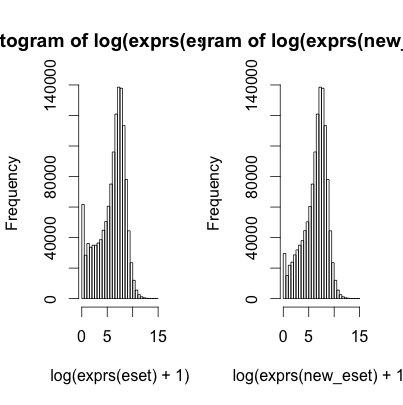
\includegraphics[width=.5\textwidth]{../../fig/histogram.png}
\caption{Histogram }
   \label{fig:histogram}
\end{figure}

% Figure: histogram of gene expression after filtering. Looks reasonably normal. 
% Figure: box-plots of the normalized data
% Figure: mean difference plots after normalization
% Figure: mean difference plots after feature selection

Comments:

The t-test that we employed to do feature selection, also known as Welch's
t-test, used the following formula:

\begin{gather}
t = \frac{\overline{X}_1-\overline{X}_2}{s_{\overline{X}_1-\overline{X}_2}} \\
s_{\overline{X}_1-\overline{X}_2} = \sqrt{\frac{s_1^2}{n_1}+\frac{s_2^2}{n_2}} \\
\text{d.f.} = \frac{\left(\frac{s_1^2}{n_1}+\frac{s_2^2}{n_2} \right)}{\frac{s_1^4}{n_1^2(n_1-1)} + \frac{s_2^4}{n_2^2(n_2-1)}}
\end{gather}

\subsection{Classification Methods}

We investigated applied a number of methods in order to classify our data:

\begin{enumerate}
\item Principal Components Analysis - Choose the genes with the top X pvalues. 
\item Support Vector Machines
\item Linear Discriminant Analysis (with two clusters)
\item Random Forests
\end{enumerate}

\subsection{Performance Metrics}

Give our classification methods, we will consider a number of performance
metrics. We will look at accuracy (total correct over all predictions). Next,
for classifiers that give probabilities, we will plot the number of correct
predictions as a function of the number of false predictions for various
thresholds. Eg. if $p>t=0.1$, we say that we cannot decide which cancer type
that patient is. 

\section{Data}

The Cancer Genome Atlas (TCGA) collects and analyzes high-quality tumor samples
and makes a variety of data available online. We have downloaded RNA seq data
for two types of cancer, KIRC and KIRP. The data was collected by the David
Neil Hayes group at UNC Chapel Hill. The data was produced using Illumina HiSeq
2000 sequencers. 

Counts per genes (GAF TCGA hg19 June 2011 build) calculated using the SeqWare
framework via the RSEM algorithm \cite{li2011rsem}.

While more data has been collected, we downloaded gene expression data from
$N_C =??$ patients with KIRC and $N_P = ??$ patients with KIRP.  For each
patient, we have gene expression data for $N_G$ genes. 

\section{Results}

After normalization and low read-count gene filtering, we produced a list of
p-values for differential expression of genes in the two cancer types. Table X
summarizes the genes with the largest p-values. Fig. Y shows a histogram of the
corrected p-values with lines showing typical significance levels. 

As in Fig. X, we plotted the scores corresponding to the first two principal
components. Evidently, the two cancer types separate nicely along the first
principal component. (Not too surprisingly since we ran this analysis using
only genes that were highly differentially expressed).  


\section{Discussion}

Our results are fundamentally limited due to the data. As this data was not
designed for this type of experiment, necessary controls are not in place. For
instance, the differences between gene expression may be due to technical
effects. The RNAseq experiments were carried out a few months apart. It is not
clear what efforts were made to standardize the procedure of processing the
cancer samples. In the future, it would be important to have a negative control
where two samples that are supposed to be the same are processed at during the
two times that the cancer cells were processed. 

\section*{Acknowledgments}

We would like to thank Davide Risso for pointing us to the Cancer Genome Atlas
as well as providing feedback on our proposal. Sandrine Dudoit and Haiyan Huang
offered us important feedback on our initial proposals as well as on our
intermediate results. 

\bibliographystyle{imsart-number} %bibliographystyle{imsart-nameyear}
\bibliography{kidney}

\end{document}
